\chapter{Introduction}	
Nowadays devices are becoming more complex. They embed several subsystems with different characteristics that communicate and interact in many ways. For example, cars can integrate an adaptive control cruise system, GPS tracking, fuel control system and soon on. Furthermore, these subsystems are widely coupled. For instance, the adaptive cruise system determines the way to get home depending on the GPS tacking, also, the fuel control system regulates the speed of the car depending on the level of fuel.
	
This makes the designing of these systems very complex. A designer has to deal with the heterogeneity of each subsystem but also with the interaction between them. To reduce the complexity of such a development, the designing is split into different domains, \eg mechanical, electronic, software. The development is thus talcked by different domains experts.
	
Model Driven Engineering (MDE) has addressed the problem of the development of application for complex systems by proposing Domain Specific Modeling Languages (DSMLs). Each domain expert relies on a DSML to better describe its domain. As a result, several models conforming to different DSMLs are developed and the specification of the overall system becomes \emph{heterogeneous}.

\todo{relajar al system designer}

\todo{relajar el hecho de que sean modelos}

\todo{Mostrar imagen de la globalization de DSMLs y con un color los actores que atacamos: system designer and language integrator}

At some point of development, these models have to be integrated to understand the system and its emerging behavior globally. A system designer has to specify how models and languages are related to each other, in both a structural and a behavioral way. In this context, the GEMOC (ANR-12-INSE-0011) initiative proposes to coordinate and disseminate the research results regarding the support of the coordinated use of various modeling languages, that is, the use of multiple modeling languages to support coordinated development of diverse aspects of a system. This thesis is part of GEMOC initiative, more precisely, we focus on the coordination~\cite{coordsignibib} of behavioral models/languages to provide simulation and/or verification capabilities for the whole system specification. 
	
Currently, Coordination Languages~\cite{coordsignibib} and Architecture Description Languages (ADLs)~\cite{frameadlsbib} provide dedicated languages to specify the coordination between particular behavioral models. This is usually done by system designers that apply some coordination patterns according to their own skills and know-how. However, in heterogeneous systems, the manual coordination of models can become tedious and error prone. To automated this task, Coordination frameworks~\cite{ptoleframebib,modhelxbib} have encoded a coordination pattern inside a tool. These approaches, however, hide the semantics of the coordination. Moreover, they rely on a general purpose language (GPL) to express the coordination. As a result, the reasoning about how a system is coordinated remains very limited.  
	
In this thesis, we deal with the coordination of heterogeneous behavioral models by leveraging on the system designer's skills. We propose a dedicated language named \bcool (standing as Behavioral Coordination Operator Language) that allows for capturing coordination patterns for a given set of DSMLs. These patterns are captured between languages, and then used to derive a coordination model automatically for models conforming to the targeted DSMLs. The coordination at the language level relies on a so-called \emph{language behavioral interface}. This interface exposes an abstraction of the language behavioral semantics in terms of Events. Thus, an integrator uses \bcool to define operators to specify how events from different language behavioral interfaces interact. These operators are defined at language level but they are applied between models to coordinate their behavior. This results in a model of coordination in \ccsl, a declarative language that describes causal and temporal relationships between events. By relying on \ccsl, we provide verification and validation of the coordinated system. All this has been implemented as a set of plugins for Eclipse as part of the GEMOC studio\footnote{http://www.gemoc.org}; which integrates technologies based on Eclipse Modeling Framework (EMF)~\footnote{http://eclipse.org/modeling/emf/} adequate for the specification of executable domain specific modeling languages. In the studio, \bcool provides coordination facilities.   

We organize the content of this thesis in six chapters. Chapter~\ref{ch:background} presents the background about the integration of structural and behavioral models. We categorize the background into approaches that compose models and approaches that coordinate models. In particular, we focus on approaches that have captured coordination pattern between languages in order to automate the coordination between models. Chapter~\ref{ch:background} sketches some requirements for a language to capture explicitly coordination patterns between languages.    

Chapter~\ref{ch:framework} presents a framework to characterize coordination pattern approaches. We use this framework to compare different approaches. From this study, we state the requirements for a language to capture coordination patterns, \ie \bcool.  

In Chapter~\ref{ch:bcool}, we elaborate on our approach by presenting \bcool. We introduce a running example: the heterogeneous model of a coffee machine. Then, we use this example all through the chapter to illustrate the syntax and semantics of \bcool. We present the current implementation in the GEMOC studio by executing and verify the coffee machine models. 

To validate our approach, we present in Chapter~\ref{ch:examples} the heterogeneous model of a surveillance video system. To coordinate these models, we propose a set of \bcool operators that capture the specification of hierarchical coordination patterns. We use this example as use case to illustrate the different steps from the specification of the coordination patterns, the coordination of a particular model and verification of the coordinated system.     

Finally, we provide the conclusion of this work, highlighting its main contributions and we give some future perspectives in Chapter~\ref{ch:conclusions}.

%\item Section~\ref{sec:coord-lang} presents the main issues in the coordination of behavioral models, and shows how they can be tackled by explicitly capturing coordination patterns at the language level. Section~\ref{sec:interfaceandexample} defines the notion of language behavioral interface by using an example language named Timed Finite State Machine (TFSM). This language is used later in Section~\ref{sec:BCOol} to illustrate \bcool. In Section~\ref{sec:caseStudies}, we validate the approach by using \bcool to capture three coordination patterns between two languages: TFSM and fUML Activities. Section~\ref{sec:related} gives an overview and comparison to related work. Section~\ref{sec:conclu} concludes with a brief summary and a discussion of ongoing and future actions.
	
%\item Finally, we provide the conclusion of this work, highlighting its main contributions and we give some future perspectives in Chapter 7.
	


%\begin{landscape}
%\begin{figure}
%	\begin{center}
%		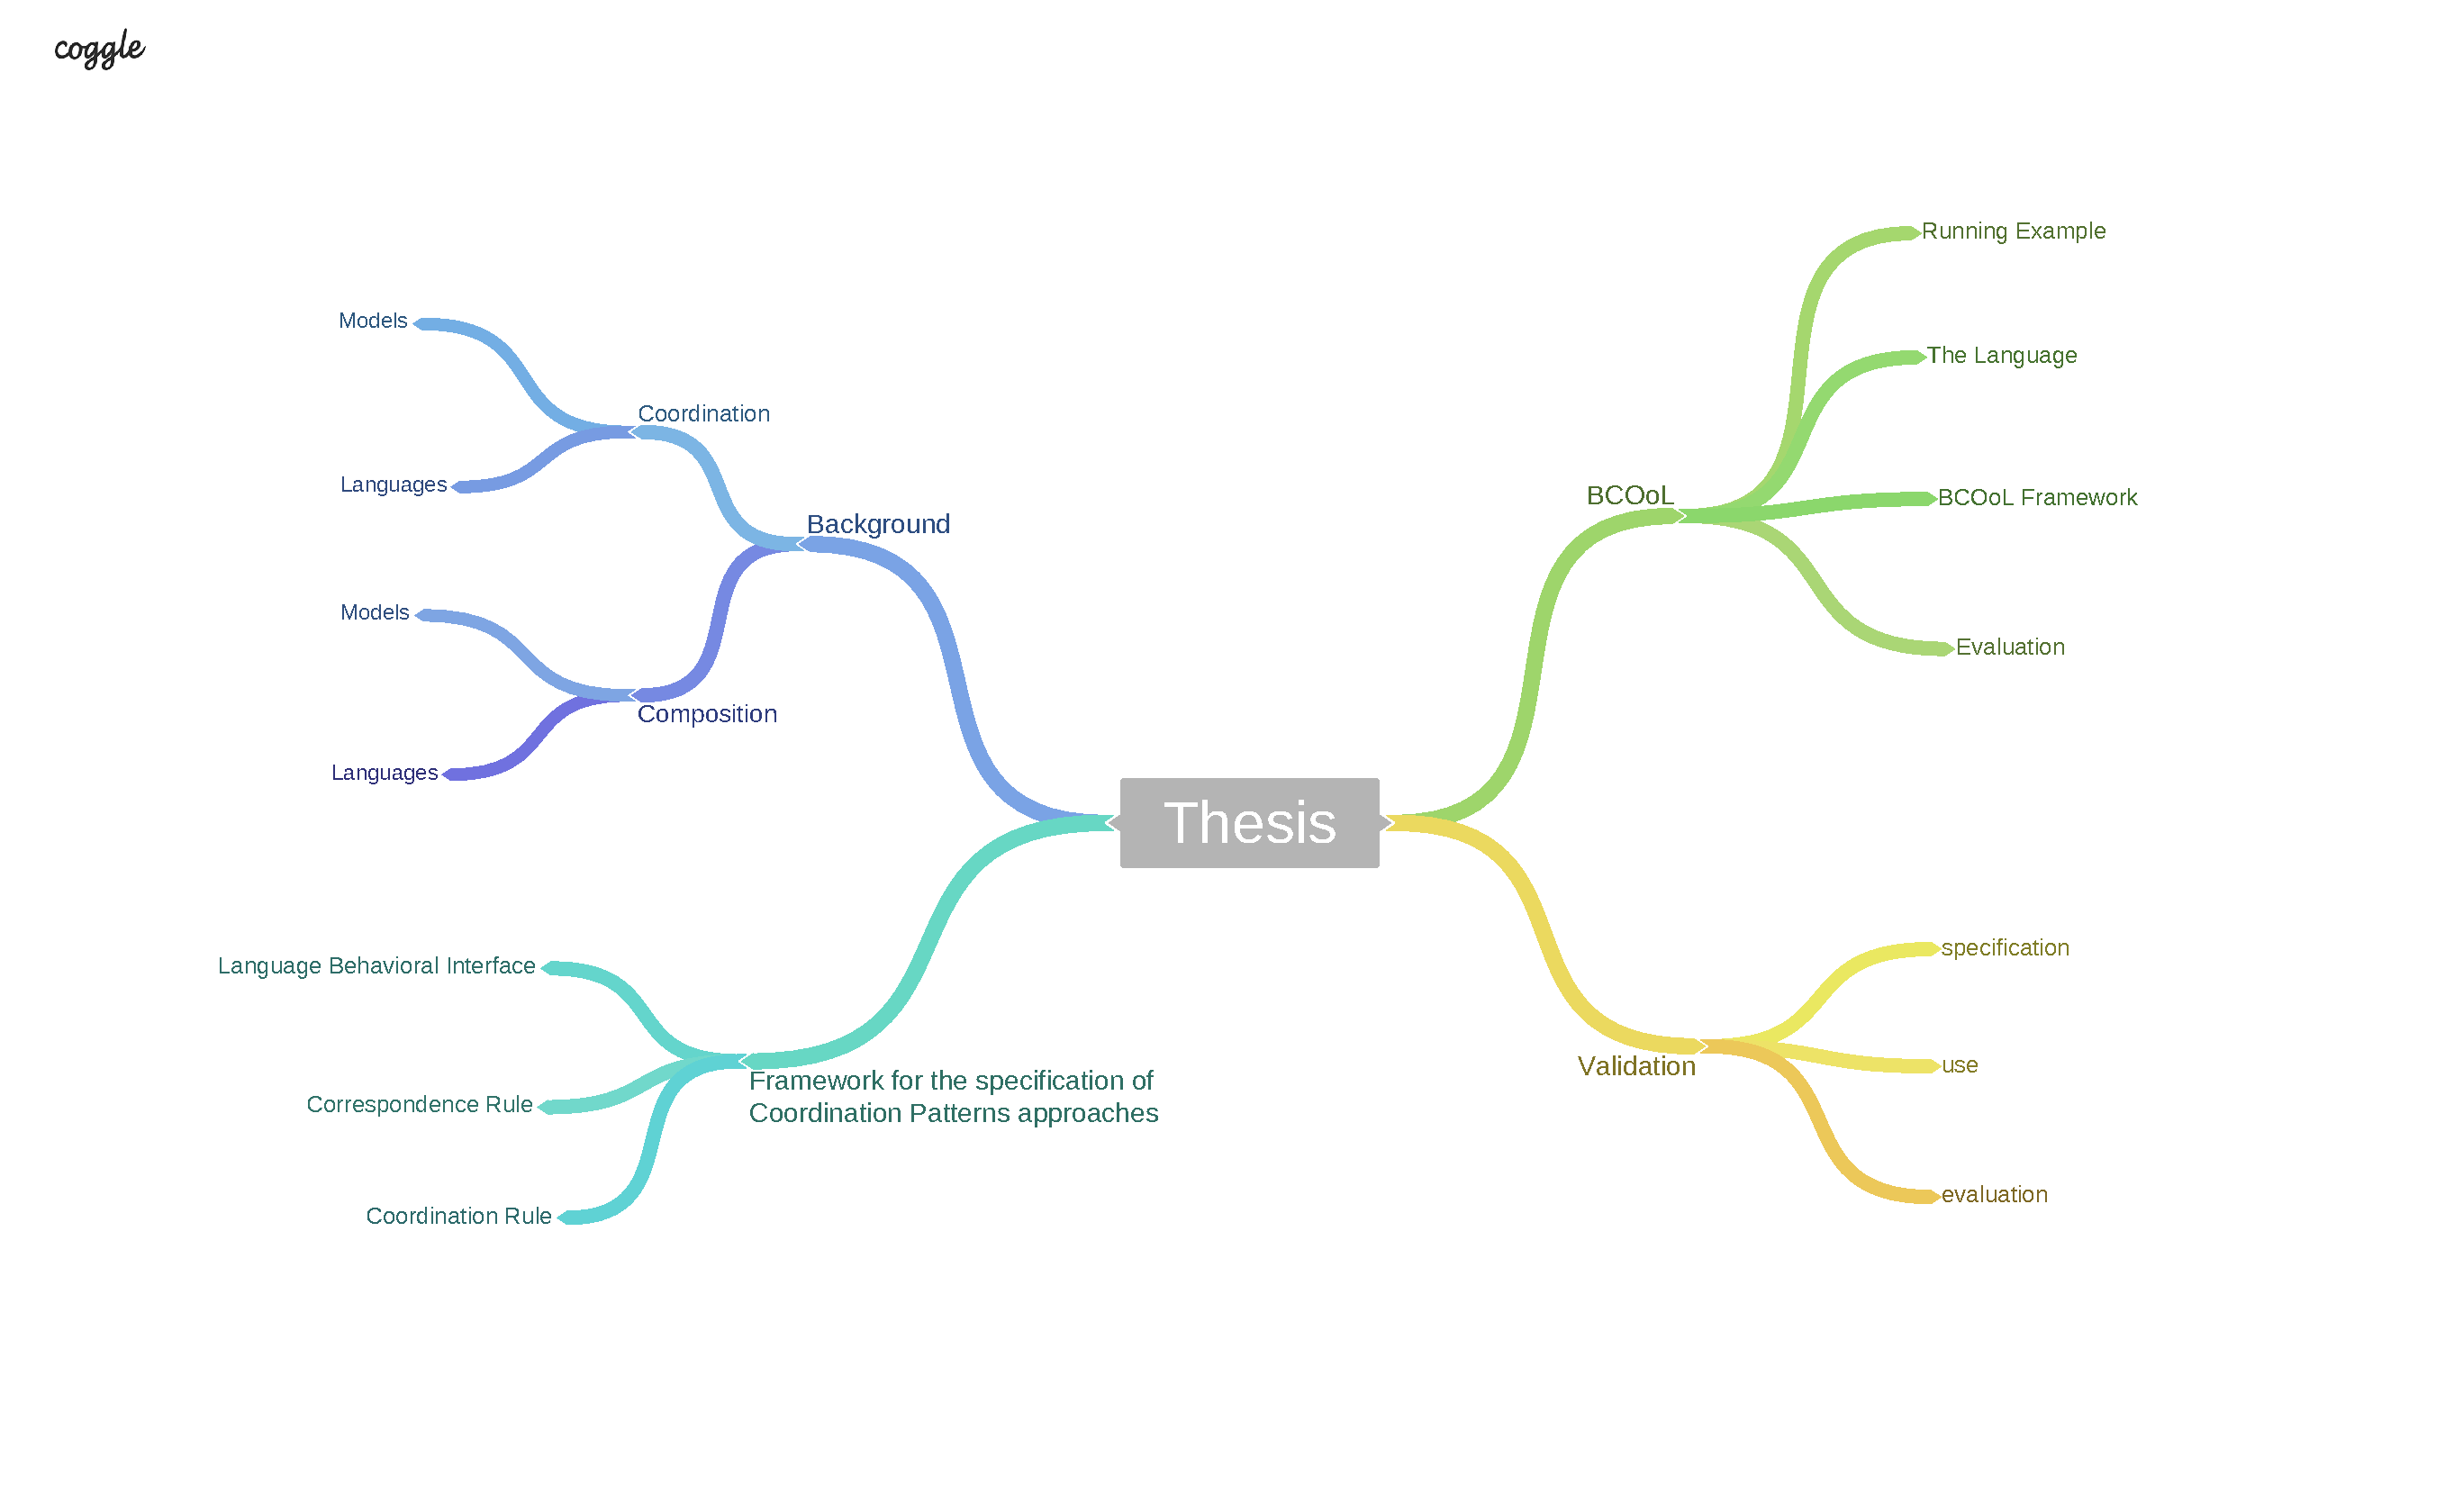
\includegraphics[width=1\textwidth]{Thesisoutline.pdf}
%		\label{fig:thesis outline}
%	\end{center}
%\end{figure}
%\end{landscape}

%\section{Problem}

%\section{Contributions}

%Contributions here.

%\section{Publications}

%Publications here.